% author: Andreas Kelbel
%
\documentclass{standalone}
% packages
  \usepackage{tikz}
	\usetikzlibrary{patterns}
	\tikzset{% 
		seil/.style={draw,color=blue,ultra thick},
		masse/.style={draw,ultra thick,fill=gray!80}
	}
  \usepackage{cmbright}		% font 
%
% macros
	\newcommand{\rolle}[4]{
		\begin{scope}[xshift=#1cm,yshift=#2cm]
			\fill[left color=gray,right color=gray!75,middle color=gray!25] (0,0) circle (.5cm) ;
			\fill[left color=gray!50, right color=gray!30, middle
			color=white] (0,0) circle (.4cm) ;
			\filldraw[fill=lightgray!50] (-.075,-#3) rectangle (.075,#4) ;
			\fill (0,0) circle (.5mm);
		\end{scope}
		}
	\newcommand{\kleinerolle}[2]{
		\begin{scope}[xshift=#1cm,yshift=#2cm]
			\fill[left color=gray,right color=gray!75,middle color=gray!25] (0,0) circle (.3cm) ;
			\fill[left color=gray!50, right color=gray!30, middle
			color=white] (0,0) circle (.2cm) ;
		\end{scope}
	}
	\newcommand{\grosserolle}[2]{
		\begin{scope}[xshift=#1cm,yshift=#2cm]
			\fill[left color=gray,right color=gray!75,middle color=gray!25] (0,0) circle (.7cm) ;
			\fill[left color=gray!50, right color=gray!30, middle
			color=white] (0,0) circle (.6cm) ;
		\end{scope}
	}
%
\begin{document}
%
  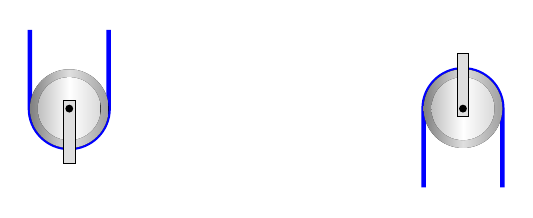
\begin{tikzpicture}
	\draw[seil] (0,0) -- (0,-1) arc(180:360:.5) -- (1,0) ;
	\rolle{.5}{-1}{.7}{.1}
	\begin{scope}[xshift=5cm,yshift=-2cm]
		\draw[seil] (0,0) -- (0,1) arc(180:0:.5) -- (1,0) ;
		\rolle{.5}{1}{.1}{.7}
	\end{scope}
  \end{tikzpicture}
    
  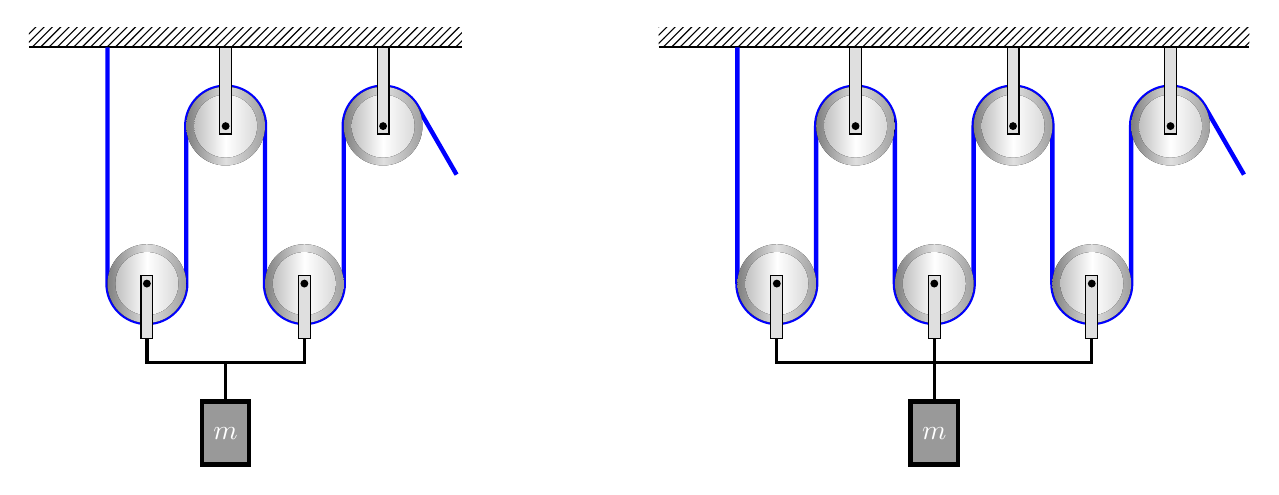
\begin{tikzpicture}
    \begin{scope}[xshift=0cm]
        \fill[pattern = north east lines] (0,0) rectangle ++(5.5,.25) ;
        \draw[thick] (0,0) -- ++(5.5,0) ;
        \draw[seil] (1,0) -- ++(0,-3) arc (180:360:.5cm) -- ++(0,2) arc (180:0:.5cm) -- ++(0,-2) arc (180:360:.5) -- ++(0,2) arc (180:30:.5) -- ++(300:1) ;
        \draw[very thick] (1.5,-3.5) -- (1.5,-4) -- ++(2,0) -- ++(0,1) (2.5,-4) -- ++(0,-1)  ;
        \rolle{1.5}{-3}{.7}{.1}
        \rolle{2.5}{-1}{.1}{1}	
        \rolle{3.5}{-3}{.7}{.1}
        \rolle{4.5}{-1}{.1}{1}	
        \fill[masse] (2.2,-4.5) rectangle ++(.6,-.8) node[midway,white]{$m$} ;
        \end{scope}
        \begin{scope}[xshift=8cm]
        \fill[pattern = north east lines] (0,0) rectangle ++(7.5,.25) ;
        \draw[thick] (0,0) -- ++(7.5,0) ;
        \draw[seil] (1,0) -- ++(0,-3) arc (180:360:.5cm) -- ++(0,2) arc (180:0:.5cm) -- ++(0,-2) arc (180:360:.5) -- ++(0,2) arc (180:0:.5) -- ++(0,-2) arc (180:360:.5) -- ++(0,2) arc (180:30:.5) -- ++(300:1) ;
        \draw[very thick] (1.5,-3.5) -- (1.5,-4) -- ++(2,0) -- ++(0,1) ++(0,-1) -- ++(2,0) -- ++(0,1) (3.5,-4) -- ++(0,-1)  ;
        \rolle{1.5}{-3}{.7}{.1}
        \rolle{2.5}{-1}{.1}{1}	
        \rolle{3.5}{-3}{.7}{.1}
        \rolle{4.5}{-1}{.1}{1}	
        \rolle{5.5}{-3}{.7}{.1}
        \rolle{6.5}{-1}{.1}{1}	
        \fill[masse] (3.2,-4.5) rectangle ++(.6,-.8) node[midway,white]{$m$} ;
      \end{scope}
	\end{tikzpicture}
%
	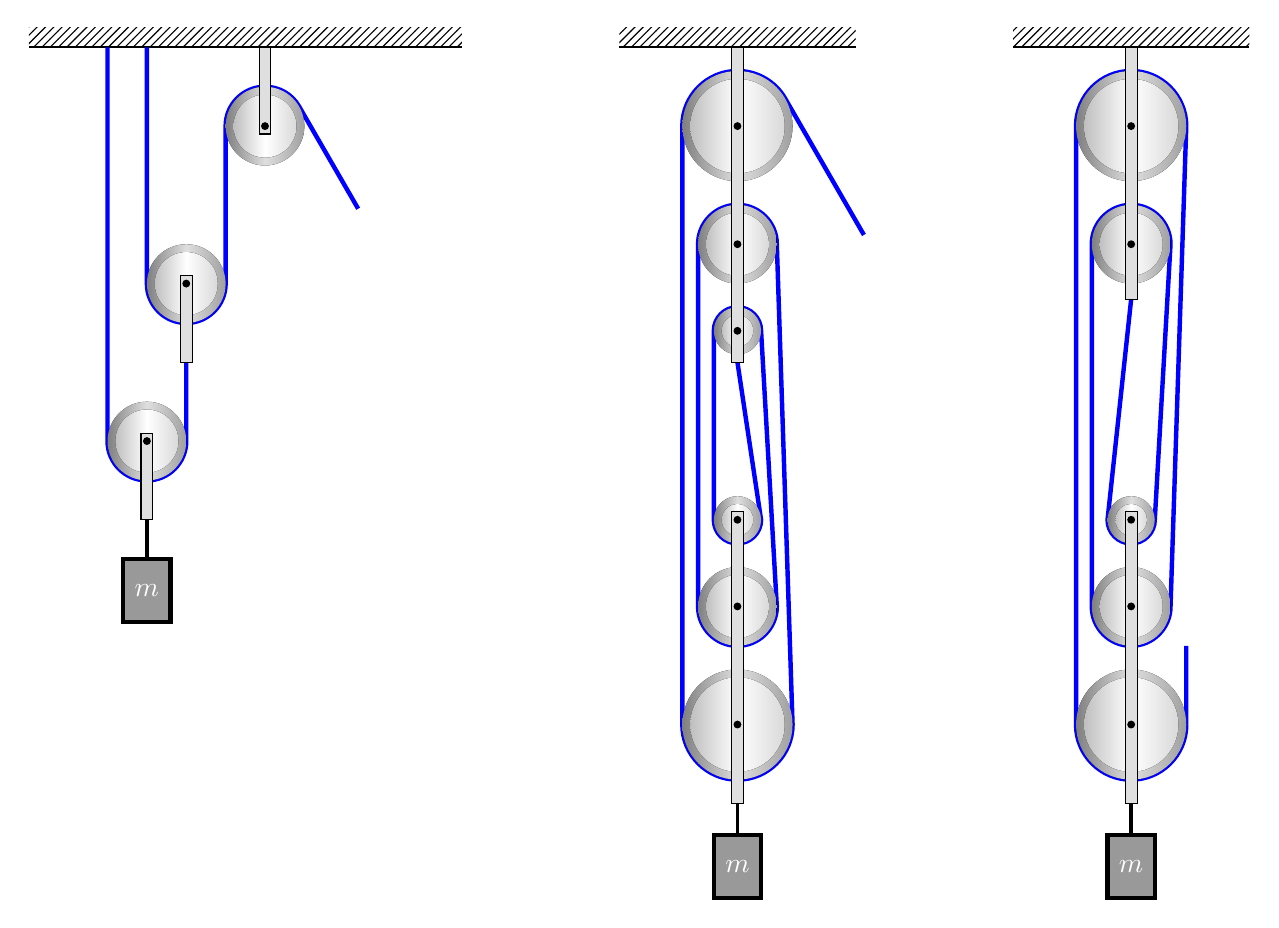
\begin{tikzpicture}
      \begin{scope}[xshift=0cm]
        \fill[pattern = north east lines] (0,0) rectangle ++(5.5,.25) ;
        \draw[thick] (0,0) -- ++(5.5,0) ;
        \draw[seil] (1,0) -- ++(0,-5) arc (180:360:.5cm) -- ++(0,1.5) ;
        \draw[seil] (1.5,0) -- ++(0,-3) arc (180:360:.5cm) -- ++(0,2) arc (180:30:.5) -- ++(300:1.5) ;
        \draw[very thick] (1.5,-6) -- ++(0,-1)  ;
        \rolle{1.5}{-5}{1}{.1}
        \rolle{2}{-3}{1}{.1}
        \rolle{3}{-1}{.1}{1}
        \fill[masse] (1.2,-6.5) rectangle ++(.6,-.8) node[midway,white]{$m$} ;
      \end{scope}
      \begin{scope}[xshift=9cm,yshift=1cm]
        \fill[pattern = north east lines] (-1.5,-1) rectangle ++(3,.25) ;
        \draw[thick] (-1.5,-1) -- ++(3,0) ;
        \draw[seil] (0,-5) -- (.3,-7) arc (360:180:.3) -- (-.3,-4.6) arc (180:0:.3) -- (.5,-8.1) arc (360:180:.5) -- (-.5,-3.5) arc (180:0:.5) -- (.7,-9.6) arc (360:180:.7) -- (-.7,-2) arc (180:30:.7) -- ++(300:2);
        \draw[very thick] (0,-10.5) -- ++(0,-1) ;

        \grosserolle{0}{-2}
        \kleinerolle{0}{-4.6}
        \rolle{0}{-3.5}{1.5}{2.5}
        \fill (0,-2) circle (.5mm);
        \fill (0,-4.6) circle (.5mm);

        \kleinerolle{0}{-7}
        \grosserolle{0}{-9.6}
        \rolle{0}{-8.1}{2.5}{1.2}
        \fill (0,-7) circle (.5mm);
        \fill (0,-9.6) circle (.5mm);

        \fill[masse] (-.3,-11) rectangle ++(.6,-.8) node[midway,white]{$m$} ;
      \end{scope}

      \begin{scope}[xshift=14cm,yshift=1cm]
        \fill[pattern = north east lines] (-1.5,-1) rectangle ++(3,.25) ;
        \draw[thick] (-1.5,-1) -- ++(3,0) ;
        \draw[seil] (0,-4.2) -- (-.3,-7) arc (180:360:.3) -- (.5,-3.5) arc(0:180:.5) -- (-.5,-8.1) arc (180:360:.5) -- (.7,-2) arc (0:180:.7) -- (-.7,-9.6) arc (180:360:.7) -- ++(90:1);
        \draw[very thick] (0,-10.5) -- ++(0,-1) ;

        \grosserolle{0}{-2}
        \rolle{0}{-3.5}{.7}{2.5}
        \fill (0,-2) circle (.5mm);

        \kleinerolle{0}{-7}
        \grosserolle{0}{-9.6}
        \rolle{0}{-8.1}{2.5}{1.2}
        \fill (0,-7) circle (.5mm);
        \fill (0,-9.6) circle (.5mm);

        \fill[masse] (-.3,-11) rectangle ++(.6,-.8) node[midway,white]{$m$} ;
      \end{scope}
	\end{tikzpicture}
\end{document} 